%%%%%%%% ICML 2021 EXAMPLE LATEX SUBMISSION FILE %%%%%%%%%%%%%%%%%

\documentclass{article}

% Recommended, but optional, packages for figures and better typesetting:
\usepackage{microtype}
\usepackage{graphicx}
\usepackage{amssymb}
\usepackage{algorithm}
\usepackage{algpseudocode}
\usepackage{inconsolata}
% \usepackage[charter]{mathdesign}
% \def\ttdefault{blg}
\usepackage{color}
\usepackage[font=footnotesize,labelfont=bf]{caption}
\usepackage[square,numbers]{natbib}
\usepackage[margin=1in]{geometry}
\usepackage{subfigure}
\usepackage{booktabs} % for professional tables
\bibliographystyle{unsrtnat}

\newcommand*{\codefont}{\fontfamily{GoMono}\selectfont}

% hyperref makes hyperlinks in the resulting PDF.
% If your build breaks (sometimes temporarily if a hyperlink spans a page)
% please comment out the following usepackage line and replace
% \usepackage{icml2021} with \usepackage[nohyperref]{icml2021} above.
\usepackage{hyperref}

% Attempt to make hyperref and algorithmic work together better:
\newcommand{\theHalgorithm}{\arabic{algorithm}}

% Use the following line for the initial blind version submitted for review:
%\usepackage{icml2021}

% If accepted, instead use the following line for the camera-ready submission:
%\usepackage[accepted]{icml2021}

% The \icmltitle you define below is probably too long as a header.
% Therefore, a short form for the running title is supplied here:
% \icmltitlerunning{Submission and Formatting Instructions for ICML 2021}

\begin{document}

\twocolumn[\centering\Large{\textbf{Parallel Implementation of Gray Level Co-occurrence Matrix Construction using MPI}}\vspace*{0.75 cm}\\ \normalsize{Aditi Jaiswal, Arianna Bunnell, and Sorapong Khongnawang}\vspace*{1 cm}]


\begin{abstract}

\end{abstract}

\section{Introduction}
    Image texture is an important feature in computer vision tasks. Textural features have been developed to allow for objective comparison of textures between images and image regions. Haralick introduced the Gray-Level Co-Occurrence Matrix (GLCM) in 1973 as a necessary step for the computation of the Haralick texture features \cite{haralick}. Constructing the GLCM for a given grayscale image involves analyzing the spatial relationships between each pixel and its neighbors for a given angle and distance \cite{haralick}. The computation of the GLCM is computationally expensive, though embarrassingly parallel, and its execution time relies heavily on the size of the image. For a grayscale image of size $n \times n$, construction of the GLCM demands $n^2$ memory accesses and $n$ writes. In this paper, we compare several methods for parallel construction of the GLCM using MPI.
\section{Background}
\subsection{Gray-Level Co-occurrence Matrix}
    Haralick devised the GLCM (referred to as Gray-Tone Spatial-Dependence Matrices in his work) as a preliminary step for the computation of the Haralick textural features \cite{haralick}. The GLCM is a flexible measure of spatial dependence between pixel gray levels which is defined by an angle, a distance, and the unique gray tones in an image. We define the GLCM for some grayscale image $A$, generally following Haralick's notation, below. \\ \\
    Suppose image $A$ has dimensions $n \times m$ pixels. If we suppose the gray level in each pixel lies within the range 0-255. We assume here the image is stored in the standard byte format, with each pixel value stored as an 8-bit integer. We let $N = \{ 1, 2, ..., n\}$ and $M = \{1, 2, ..., m\}$ be the spatial coordinates of the pixels along the vertical and horizontal domains, respectively. Thus, the set $N \times M $ represents all spatial coordinates in the image $A$. Each spatial coordinate maps to a single gray level. We then arrive at the following mapping which defines the gray tones in an image: $ A:  N \times M \to G$, where $G$ is the set of all gray tones. \\ \\
    The GLCM is a matrix of frequencies. We record the frequency that each pair of gray tones $g_e$ and $g_f$ occur within some distance $d$ of each other, at some angle $a$, where $g_e, g_f \in G$, $a \in \{0, 45, 90, 135\}$ and $d \in \{1, 2, ..., \min(m, n)\}$. Thus, GLCM $\in \mathbb{N}^{c \times c}$ where $c$ is the cardinality of the set $G$ for our given image $A$. The angle $a$ defines along which axis we walk the distance $d$ and is pictured in Figure \ref{fig:directions}. Each pixel $p$ in an image then has 8 possible neighboring pixels, excluding those for which these neighbors would extend beyond the edge of the grayscale image $A$. \\ \\
    \begin{figure}
      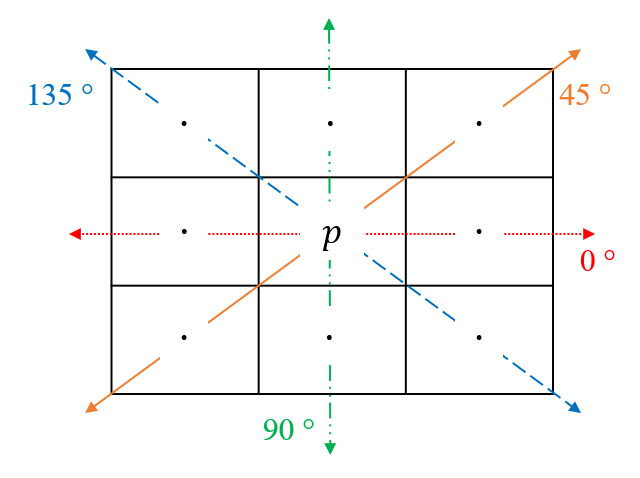
\includegraphics[width=\linewidth]{direction_fig.PNG}
      \caption{If we consider a certain pixel $p$ from a certain grayscale image $A$, we can define the angle-dependent spatial relationships as shown. Each arrow represents the line on which we compute $d-$distance nearest neighbors from our pixel $p$. The red, dotted line shows the 0\textdegree  path; the orange, solid line shows 45\textdegree  path; the green, dotted and dashed line shows the 90\textdegree  path, and the blue, dashed line shows the 135\textdegree  path. Adapted from: Robert Haralick, K. Shanmugam, and Ih Dinstein. Textural features for image classification. \textit{IEEE Trans Syst Man Cybern}, SMC-3:610–621, 01 1973. }
      \label{fig:directions}
    \end{figure}
        The choice of angle $a$ and distance $d$ for a certain image is dependent on the type of texture being classified. Coarse textures are better represented with a large distance and fine textures are better represented with a small distance. Typically, the GLCM of distance $d$ will be computed for all angles $a$, unless there is some prior knowledge about what direction the texture in $A$ should fall. \\ \\
       Figure \ref{fig:matrix} shows an example computation of a GLCM for some image $A$, depicted in Figure \ref{fig:matrix}(a) with distance 1 ($d = 1$). Figure \ref{fig:matrix}(b) shows the coordinate system for a general image where there are six gray tone values. Each cell is filled with the frequency at which the coordinate gray tones appear as neighbors, given a particular distance and angle. Figure \ref{fig:matrix}(c)-(f) show GLCMs constructed from $A$ using each possible value for the angle at distance 1. For example, Figure \ref{fig:matrix}(e) shows the GLCM constructed from $A$ when $a = 90$ and $d = 1$. The elements (0,3) and (3,0) reflect that the gray tones 0 ad 3 appear next to one another on the vertical angle line one time. Note that, as defined by Haralick, a GLCM will always be symmetric. 
    \begin{figure}[t]
      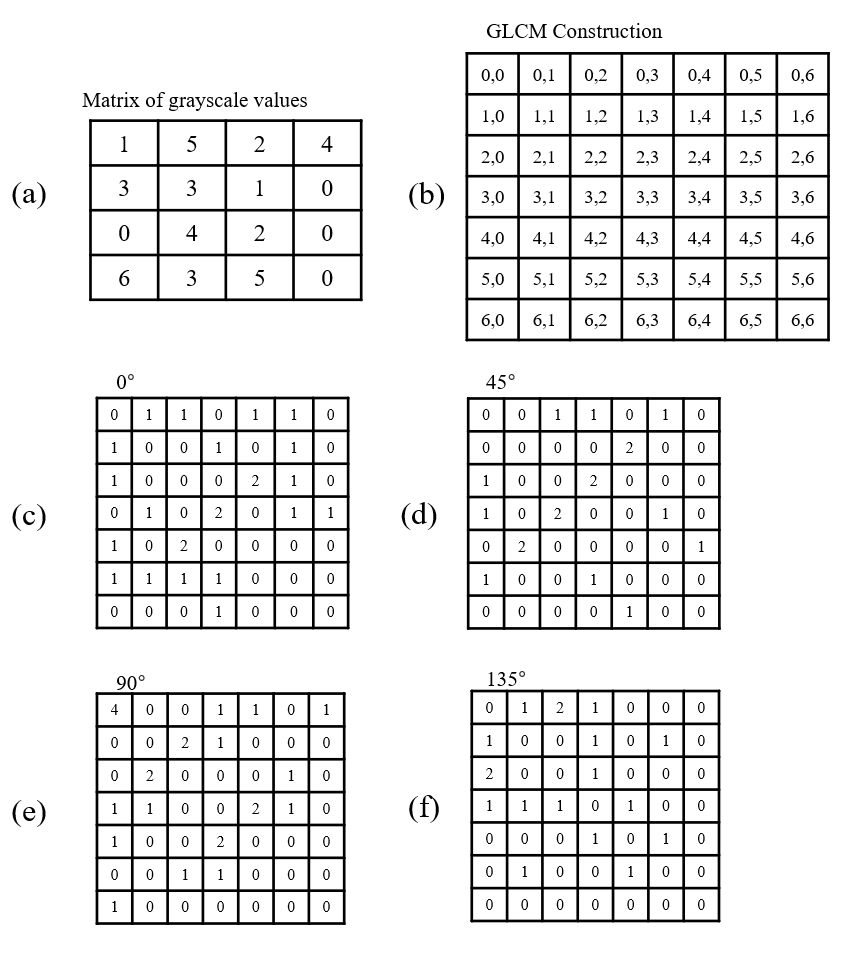
\includegraphics[width=\linewidth]{matrix_fig.PNG}
      \caption{ (a) a $4 \times 4$ image $A$ with six gray tones, $G = \{0, 1, 2, 3, 4, 5, 6\}$. (b) General form of any GLCM constructed from $A$, or any other image with 6 gray tones. The coordinate system is $G \times G$. (c)-(f) GLCMs for angle values (clockwise from top right) 0, 45, 135, and 90 degrees at $d = 1$ for our image $A$.  Adapted from: Robert Haralick, K. Shanmugam, and Ih Dinstein. Textural features for image classification. \textit{IEEE Trans Syst Man Cybern}, SMC-3:610–621, 01 1973. }
      \label{fig:matrix}
    \end{figure}
\subsection{MPI}
   MPI is a standard message passing interface
   designed for distributed memory systems. MPI was first proposed in 1993 as the culmination of efforts from more than 40 organizations from  the United States and across Europe \cite{mpi1}. MPI is now the standard for distributed memory systems. MPI provides routines for both blocking and non-blocking communication between processes, and routines for collective communication between all processes \cite{mpi}. \\ \\ 
   We do not provide a comprehensive review of MPI here, but simply outline the communication routines which we make use of in our implementation. \texttt{MPI\_Send} represents a blocking send procedure. A single envelope of data is sent from process $x$ to process $y$. The program cannot continue until process $y$ acknowledges receipt of the envelope. \texttt{MPI\_Recv} represents a blocking receive procedure. After process $x$ sends its envelope, process $y$ must wait until it receives the envelope from process $x$ to proceed.  \\ \\ 
   MPI allows for computation over a large set of data to be distributed over many processes. We use MPI to partition out the image $A$. Each process independently constructs a section of the GLCM. A single root process then gathers the partial GLCMs computed by the processes and combines them into a single GLCM for the image $A$. 
\section{Related Work}
    The literature focused on implementing parallel versions of  the Haralick texture features tends to also include information on parallelization of GLCM construction. Parallel implementations and hardware-specific implementations are of specific interest in the medical field, where Haralick features are used for analysis of medical imaging \cite{medref1} \cite{medref2} \cite{medref3} \cite{medref4}. Efficient parallel implementations of GLCM construction is needed for both 2D and 3D medical imaging modalities. \\ \\ 
    HaraliCU is an algorithm which exploits the parallel computation capabilities of Graphics Processing Units (GPUs) to efficiently compute the Haralick features \cite{haralicpu}. HaraliCU computes the GLCM using a sliding window approach. Each pixel of a sliding window of the image $A$ is assigned to a single thread, and its neighbors within that window are computed before moving to the next window. The GLCM is stored as a flat list, with entries $(g_e, g_f), freq$ where $(g_e, g_f) \in G \times G$ and $freq$ represents the frequency of the given spatial relationship between $g_e$ and $g_f$ occurring. The HaraliCPU implementation achieved a 15.90$\times$ speedup on multi-threaded GPUs over a sequential version on a single CPU  \cite{haralicpu}. HaraliCPU depends on the fact that GPU is available and also does not make use of shared memory, causing unnecessary latencies. \\ \\ 
    Another exploration into using GPUs to achieve highly parallel computation of the Haralick features is found in \cite{gipp}. Gipp et al. examined parallelization of GLCM construction and feature computation on microscopy images. Due to the relative simplicity of gray tone spatial relationships in microscopy imagery (typically only 2 or 3 unique neighboring gray tones)  Gipp et al. chose to condense the GLCM by removing all zero-filled rows and columns \cite{gipp}. It's unclear how effective the "packing" strategy would be on an image with more variation in its spatial relationships. Gipp et al. also implement parallelization by splitting their multi-cell microscopy images into single- cell images, and passing each image to a separate GPU thread \cite{gipp}. Gipp et al. do not use distributed memory in their approach, and do not implement parallelization on the individual image level. \\ \\
   Parallel GLCM construction using distributed memory is seen in \cite{shahbahrami}. Shahbahrami, Pham, and Bertels implement GLCM construction and computation of the Haralick texture features in parallel on a cell architecture, a multi-core architecture containing nine processors of two types \cite{shahbahrami}.  Shahbahrami, Pham, and Bertels achieved a 10$\times$ speedup over non-parallel optimized implementations. Shahbahrami, Pham, and Bertels approach GLCM construction similarly to our method, splitting the image by rows to compute independently, before summing at two levels (i.e. for four processes, a sum is computed between processes 1 and 2 in parallel with processes 3 and 4, then a final sum is computed) to construct the final GLCM \cite{shahbahrami}. Shahbahrami, Pham, and Bertels tested their implementation with images with only 128 distinct gray levels, limiting the real-world implications of their results. 
\section{Parallel Algorithm}
    We implemented two different parallel implementations of the GLCM construction process. Each algorithm makes use of MPI processes having their own memory to store partial computations and a partial copy of the grayscale image, while referring to a relevant section of the grayscale image $A$. We implemented a row-based parallel algorithm, a tiled parallel algorithm, and a sequential algorithm. \\ \\ 
    The row-based parallel algorithm computes the GLCM for a particular combination of a grayscale image $A$, an angle $a$, a distance $d$ and a number of processes $X$. We restrict the number of processes to an integer factor of the number of rows in the image ($N$) to simplify partitioning. Each process needs to compute a partial GLCM based on the pixels in $\frac{N}{X}$ rows of the image $A$. \\ \\ 
    We define the root process as $P_0$. The root process reads in the entire grayscale image $A$ and computes the number of gray levels in the image ($G$). The root then performs an \texttt{MPI\_Bcast} to share the size ($G \times G$) with the workers. Each worker process $P_x$ where $x \in X / \{0\}$ receives rows $x \cdot \frac{N}{X} - d$ to $x \cdot \frac{N}{X} + d$ from the root process $P_0$ and allocates a partial GLCM of size $G \times G$. Then, the root process receives all partial GLCMs from the worker processes and computes the final GLCM for the entire image $A$. The algorithm for the child processes is displayed in Algorithm \ref{alg:1} and the algorithm for the root process is displayed in Algorithm \ref{alg:2}. \\ \\ 
    The tiled parallel algorithm computes the GLCM for a particular combination of a grayscale image $A$, an angle $a$, a distance $d$ and a number of processes $X$. We restrict the number of processes to an integer factor of the number of rows in the image ($N$) to simplify partitioning, and require the image size to be $N \times N$.
\begin{algorithm}
    \caption{Algorithm for the non-root MPI processes, $P_x$ where $x \in X$ and $x > 0$. $X$ is the total number of processes. Note that partial rows here is not an exact translation from the code. Partial rows in the  \texttt{MPI\_Receive} is the total set of rows needed to compute neighbors, while partial rows in the for loop is the rows we are computing for. }\label{alg:1}
    \begin{algorithmic}
       % \Require $n \geq 0$
       % \Ensure $y = x^n$
    %    \State $start \gets x \cdot \frac{N}{X}$
    %    \State $stop \gets (x + 1) \cdot \frac{N}{X}$
        \State \texttt{MPI\_Bcast}$($GLCM\_size$, P_0)$
        \State partial $\gets [0, 0, 0, ..., 0]$
        \State partial image $\gets $  \texttt{MPI\_Receive}$($partial image$, P_0)$ \\
        \While{$p$ in partial image} 
        \If{$p$ has a neighbor}
            \State partial$[g_{n}][g_p] \gets $partial$[g_{n}][g_p] + 1$
           % \State $N \gets \frac{N}{2}$  \Comment{This is a comment}
        \EndIf
        \EndWhile \\
        \State \texttt{MPI\_Send}$($partial$, 0)$
    \end{algorithmic}
\end{algorithm}

\begin{algorithm}
    \caption{Algorithm for the root MPI process, $P_0$. }\label{alg:2}
    \begin{algorithmic}
        \State GLCM $\gets [0, 0, 0, ..., 0]$
        \State \texttt{MPI\_Bcast}$($GLCM\_size$, P_0)$ \\ 
        \While{$p$ in GLCM}
        \If{$p$ has a neighbor}
            \State $GLCM[p] \gets GLCM[p] + 1$
        \EndIf
        \EndWhile \\
        \For{$x := 1$ \textbf{to} $X$}
            \State \texttt{MPI\_Receive}$($partial$, P_x)$
            \State $GLCM \gets $GLCM + partial
        \EndFor
    \end{algorithmic}
\end{algorithm}

\section{Experimental Results}
\subsection{Simulated Experiments}
\subsection{Cluster Experiments}

\section{Conclusion }

\bibliography{references}

% The style file uses the \texttt{hyperref} package to make clickable
% links in documents. If this causes problems for you, add
% \texttt{nohyperref} as one of the options to the \texttt{icml2021}
% usepackage statement.





% \begin{figure}[ht]
% \vskip 0.2in
% \begin{center}
% \centerline{\includegraphics[width=\columnwidth]{icml_numpapers}}
% \caption{Historical locations and number of accepted papers for International
% Machine Learning Conferences (ICML 1993 -- ICML 2008) and International
% Workshops on Machine Learning (ML 1988 -- ML 1992). At the time this figure was
% produced, the number of accepted papers for ICML 2008 was unknown and instead
% estimated.}
% \label{icml-historical}
% \end{center}
% \vskip -0.2in
% \end{figure}

% \subsection{Figures}

% You may want to include figures in the paper to illustrate
% your approach and results. Such artwork should be centered,
% legible, and separated from the text. Lines should be dark and at
% least 0.5~points thick for purposes of reproduction, and text should
% not appear on a gray background.

% Label all distinct components of each figure. If the figure takes the
% form of a graph, then give a name for each axis and include a legend
% that briefly describes each curve. Do not include a title inside the
% figure; instead, the caption should serve this function.

% Number figures sequentially, placing the figure number and caption
% \emph{after} the graphics, with at least 0.1~inches of space before
% the caption and 0.1~inches after it, as in
% Figure~\ref{icml-historical}. The figure caption should be set in
% 9~point type and centered unless it runs two or more lines, in which
% case it should be flush left. You may float figures to the top or
% bottom of a column, and you may set wide figures across both columns
% (use the environment \texttt{figure*} in \LaTeX). Always place
% two-column figures at the top or bottom of the page.

% \subsection{Citations and References}

% Please use APA reference format regardless of your formatter
% or word processor. If you rely on the \LaTeX\/ bibliographic
% facility, use \texttt{natbib.sty} and \texttt{icml2021.bst}
% included in the style-file package to obtain this format.

% Citations within the text should include the authors' last names and
% year. If the authors' names are included in the sentence, place only
% the year in parentheses, for example when referencing Arthur Samuel's
% pioneering work \yrcite{Samuel59}. Otherwise place the entire
% reference in parentheses with the authors and year separated by a
% comma \cite{Samuel59}. List multiple references separated by
% semicolons \cite{kearns89,Samuel59,mitchell80}. Use the `et~al.'
% construct only for citations with three or more authors or after
% listing all authors to a publication in an earlier reference \cite{MachineLearningI}.

% Authors should cite their own work in the third person
% in the initial version of their paper submitted for blind review.
% Please refer to Section~\ref{author info} for detailed instructions on how to
% cite your own papers.

% Use an unnumbered first-level section heading for the references, and use a
% hanging indent style, with the first line of the reference flush against the
% left margin and subsequent lines indented by 10 points. The references at the
% end of this document give examples for journal articles \cite{Samuel59},
% conference publications \cite{langley00}, book chapters \cite{Newell81}, books
% \cite{DudaHart2nd}, edited volumes \cite{MachineLearningI}, technical reports
% \cite{mitchell80}, and dissertations \cite{kearns89}.

% Alphabetize references by the surnames of the first authors, with
% single author entries preceding multiple author entries. Order
% references for the same authors by year of publication, with the
% earliest first. Make sure that each reference includes all relevant
% information (e.g., page numbers).

% Please put some effort into making references complete, presentable, and
% consistent. If using bibtex, please protect capital letters of names and
% abbreviations in titles, for example, use \{B\}ayesian or \{L\}ipschitz
% in your .bib file.

% \section*{Software and Data}

% If a paper is accepted, we strongly encourage the publication of software and data with the
% camera-ready version of the paper whenever appropriate. This can be
% done by including a URL in the camera-ready copy. However, \textbf{do not}
% include URLs that reveal your institution or identity in your
% submission for review. Instead, provide an anonymous URL or upload
% the material as ``Supplementary Material'' into the CMT reviewing
% system. Note that reviewers are not required to look at this material
% when writing their review.

% % Acknowledgements should only appear in the accepted version.
% \section*{Acknowledgements}

% \textbf{Do not} include acknowledgements in the initial version of
% the paper submitted for blind review.

% If a paper is accepted, the final camera-ready version can (and
% probably should) include acknowledgements. In this case, please
% place such acknowledgements in an unnumbered section at the
% end of the paper. Typically, this will include thanks to reviewers
% who gave useful comments, to colleagues who contributed to the ideas,
% and to funding agencies and corporate sponsors that provided financial
% support.


% % In the unusual situation where you want a paper to appear in the
% % references without citing it in the main text, use \nocite
% \nocite{langley00}

% \bibliography{example_paper}
% \bibliographystyle{icml2021}


% %%%%%%%%%%%%%%%%%%%%%%%%%%%%%%%%%%%%%%%%%%%%%%%%%%%%%%%%%%%%%%%%%%%%%%%%%%%%%%%
% %%%%%%%%%%%%%%%%%%%%%%%%%%%%%%%%%%%%%%%%%%%%%%%%%%%%%%%%%%%%%%%%%%%%%%%%%%%%%%%
% % DELETE THIS PART. DO NOT PLACE CONTENT AFTER THE REFERENCES!
% %%%%%%%%%%%%%%%%%%%%%%%%%%%%%%%%%%%%%%%%%%%%%%%%%%%%%%%%%%%%%%%%%%%%%%%%%%%%%%%
% %%%%%%%%%%%%%%%%%%%%%%%%%%%%%%%%%%%%%%%%%%%%%%%%%%%%%%%%%%%%%%%%%%%%%%%%%%%%%%%
% \appendix
% \section{Do \emph{not} have an appendix here}

% \textbf{\emph{Do not put content after the references.}}
% %
% Put anything that you might normally include after the references in a separate
% supplementary file.

% We recommend that you build supplementary material in a separate document.
% If you must create one PDF and cut it up, please be careful to use a tool that
% doesn't alter the margins, and that doesn't aggressively rewrite the PDF file.
% pdftk usually works fine. 

% \textbf{Please do not use Apple's preview to cut off supplementary material.} In
% previous years it has altered margins, and created headaches at the camera-ready
% stage. 
% %%%%%%%%%%%%%%%%%%%%%%%%%%%%%%%%%%%%%%%%%%%%%%%%%%%%%%%%%%%%%%%%%%%%%%%%%%%%%%%
% %%%%%%%%%%%%%%%%%%%%%%%%%%%%%%%%%%%%%%%%%%%%%%%%%%%%%%%%%%%%%%%%%%%%%%%%%%%%%%%


\end{document}


% This document was modified from the file originally made available by
% Pat Langley and Andrea Danyluk for ICML-2K. This version was created
% by Iain Murray in 2018, and modified by Alexandre Bouchard in
% 2019 and 2021. Previous contributors include Dan Roy, Lise Getoor and Tobias
% Scheffer, which was slightly modified from the 2010 version by
% Thorsten Joachims & Johannes Fuernkranz, slightly modified from the
% 2009 version by Kiri Wagstaff and Sam Roweis's 2008 version, which is
% slightly modified from Prasad Tadepalli's 2007 version which is a
% lightly changed version of the previous year's version by Andrew
% Moore, which was in turn edited from those of Kristian Kersting and
% Codrina Lauth. Alex Smola contributed to the algorithmic style files.